\newpage
\onecolumn
\section*{Frequently Asked Questions (FAQs)}\label{sec:FAQs}

\begin{itemize}
[leftmargin=2mm]
\setlength\itemsep{0em}
    \item[\ding{93}] {\fontfamily{lmss} \selectfont \textbf{This study explores the unintended, negative aspects of hallucination; how about the useful effects that arise as a result of hallucination?}}
    \vspace{-2mm}
    \begin{description}
    \item[\ding{224}] While hallucinating has beneficiary effects in some computer vision use cases, where a generative vision model could perform in-painting of an occluded content in an image or generate an image of a scenario it hasn't seen in its training set (for example, a generated image corresponding to the prompt, ``water on Mars''), but it is usually undesirable in the context of the text. The downstream impact as a result of the model's is exacerbated by the fact that there is a lack of a programmatic method in the research community to distinguish the hallucinated vs. factually correct output. For this reason, this study focuses on characterizing the problem of hallucination particularly in the context of text.
    \end{description}

    \item[\ding{93}] {\fontfamily{lmss} \selectfont \textbf{Why do you select those 15 large language models?}}
    \vspace{-2mm}
    \begin{description}
    \item[\ding{224}] We want to select several language models with varying parameter sizes for our experiments - ranging from large to small. Hence, the above chosen 14 models consist of large models like GPT-3 and smaller ones like T5 and T0.
    \end{description}

    \item[\ding{93}] {\fontfamily{lmss} \selectfont \textbf{Why would extrinsic hallucination be riskier?}}
    \vspace{-2mm}
    \begin{description}
    \item[\ding{224}] According to the ``extrinsic hallucination'' definition, this kind of hallucination does not have any way to verify it from the source prompt. Hence, it is likely to be more harmful than the intrinsic ones.
    \end{description}

    \item[\ding{93}] {\fontfamily{lmss} \selectfont \textbf{What is the purpose of constructing Factual Mirage and Silver Lining  hallucination data?}}
    \vspace{-2mm}
    \begin{description}
    \item[\ding{224}] We want to show that hallucinations can happen in both cases, factually correct and incorrect prompts. Hence, in this paper, we construct an exhaustive dataset called 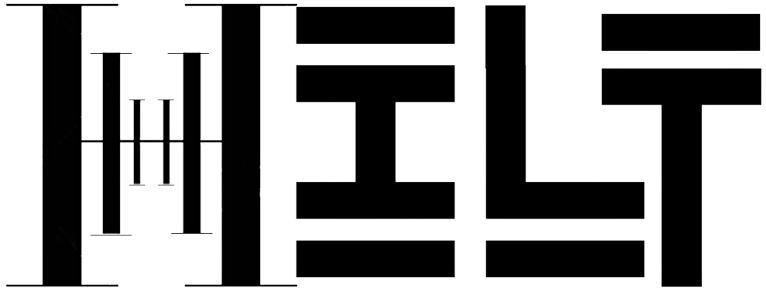
\includegraphics[height=0.3cm,width=1cm]{img/hilt.png}.
    \end{description}

    \item[\ding{93}] {\fontfamily{lmss} \selectfont \textbf{Why do you select high-entropy points for mitigation techniques?}}
    \vspace{-2mm}
    \begin{description}
    \item[\ding{224}] High entropy points are more uncertain points in the context of text generation and hence, more likely places where the LLM hallucinates. Hence, our mitigation approach works by detecting and replacing such high entropy points.
    \end{description}

    \item[\ding{93}] {\fontfamily{lmss} \selectfont \textbf{Why would HVI be a better hallucination evaluation metric for the LLMs (as compared to the existing ones like accuracy, precision, recall, F1, etc.)?}}
    \vspace{-2mm}
    \begin{description}
    \item[\ding{224}] Although the commonly used evaluation metrics like accuracy, precision, etc. can be used for downstream tasks, HVI can be more specifically used to determine the LLMs' hallucination tendency. HVI will serve as a uniform hallucination score for all the present and future LLMs.
    \end{description}

    \item[\ding{93}] {\fontfamily{lmss} \selectfont \textbf{What are the insights on using black-box vs. gray-box models for mitigation hallucinations?}}
    \vspace{-6mm}
    \begin{description}
    \item[\ding{224}] Both black-box and gray-box models have their own advantages and disadvantages in terms of reducing hallucinations. Therefore, the choice of the appropriate method to minimize hallucination would be LLM- and task-dependent.
    \end{description}

\end{itemize}    